%!TEX root =  ../final-report.tex

% Chapters are setup to start on a new page.
% The short version of that title appears in square brackets. This is used for the table of contents listing. 
% The long version of the title has a command "\setstretch{0.5}" in order to reduce the line spacing in the
% title and then the title text.

\chapter{Multiplexer}
\label{sec:Multiplexer}

The multiplexer consists of two sections; an RF switch section and a DC switch section. The RF switch provides a path for the signal to and from the VNA to the antennas, while the DC switch provides the logic necessary to set the correct path in the RF switch at the correct time. In order to collect the data required to create an image of the grain bins contents, an array of antennas needs to be connected to the VNA. Figure \ref{fig:mp_connections} shows how the multiplexer connects the VNA to the array of antennas. The VNA has two ports, one which transmits a signal and one which receives a signal. Through commands sent from the DC switch, the multiplexer is capable of connecting either of these two ports to any of the antennas in the array.

\section{RF Switch}

\subsection{Background}

The multiplexer must connect the ports from the VNA in a certain sequence. First, the multiplexer will be configured to connect the transmitter port from the VNA to antenna 1. After this, antenna 2 will be connected to the receiver port of the VNA. Then antenna 3 connects to the receiver port, then antenna 4 and so on through the entire array of antennas. Once this sequence has been completed the multiplexer will now be configured to connect the transmitter port of the VNA to antenna 2, after which antenna 1 will be connected to the receiver port, then antenna 3, then antenna 4 and so on through the entire array again. The multiplexer will repeat this sequence until all antennas have acted as the transmitter with the remaining antennas acting as receivers.

\begin{figure}[h]
	\begin{center}
		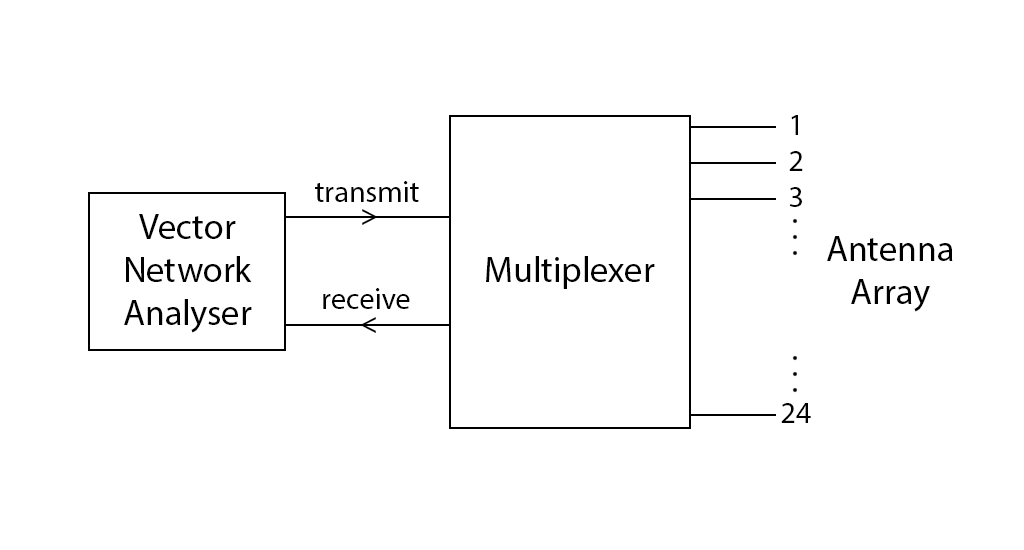
\includegraphics[width=4.5in]{./images/multiplexer_connections.png}
		\caption{Multiplexer connecting VNA to antenna array}
		\label{fig:mp_connections}
	\end{center}
\end{figure}

\subsection{Design}

An initial design for the RF multiplexer was created using six 4 x 2 matrix switches together two SP3Ts. The topology of this design is shown in figure \ref{fig:mp_initial_layout}. Note that not all of the 4 x 2 matrix switches are shown in the figure, 4 more of these switches are connected to the two remaining pins of the two SP3Ts for a total of 24 antennas. The 4 x 2 matrix switch chosen for this design was from Hittite Microwave Corporation, part number HMC596LP4 and the SP3Ts chosen were part number HMC245QS16 also from Hittite Microwave Corporation.  This design was chosen for its simplicity which would allow for good performance.

However, we were not able to use this design, as it was realized that the 4 x 2 matrix switches chosen do not operate in the frequency range needed for our project of 70 - 90 MHz. More research was done but no switches of this type were found that operate in the required frequency range for this project. Due to this limitation a new design was chosen consisting of a series of cascaded RF switches, including SPDTs, SP3Ts and SP8Ts. The topology of this design is shown in figure \ref{fig:mp_final_layout}. The switches used in this design are HMC349MS8G, HMC245QS16 and HMC253QS24 from Hittite Microwave Corporation.


\begin{figure}[h]
	\begin{center}
		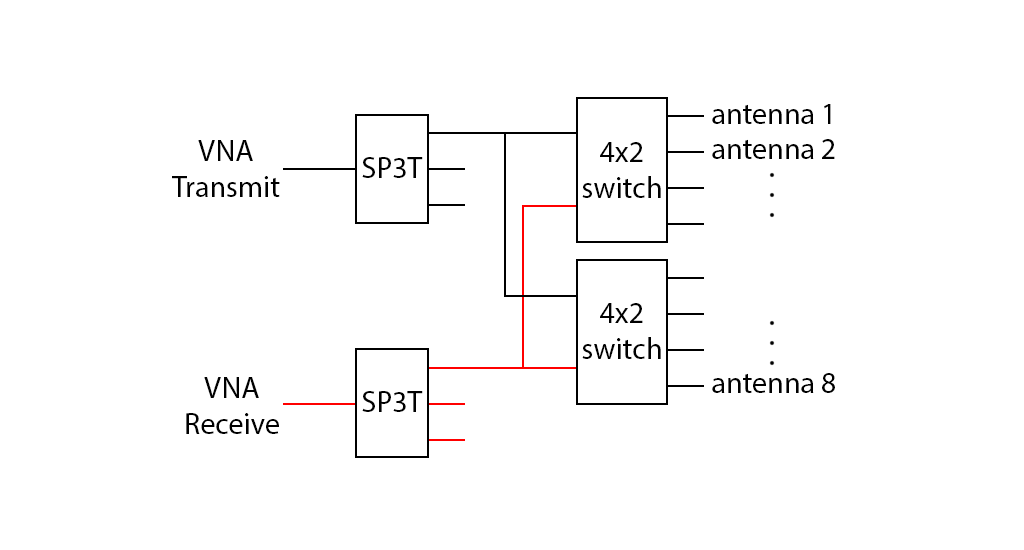
\includegraphics[width=5in]{./images/mp_initial_layout.png}
		\caption{Initial design of the multiplexer}
		\label{fig:mp_initial_layout}
	\end{center}
\end{figure}

\begin{figure}[h]
	\begin{center}
		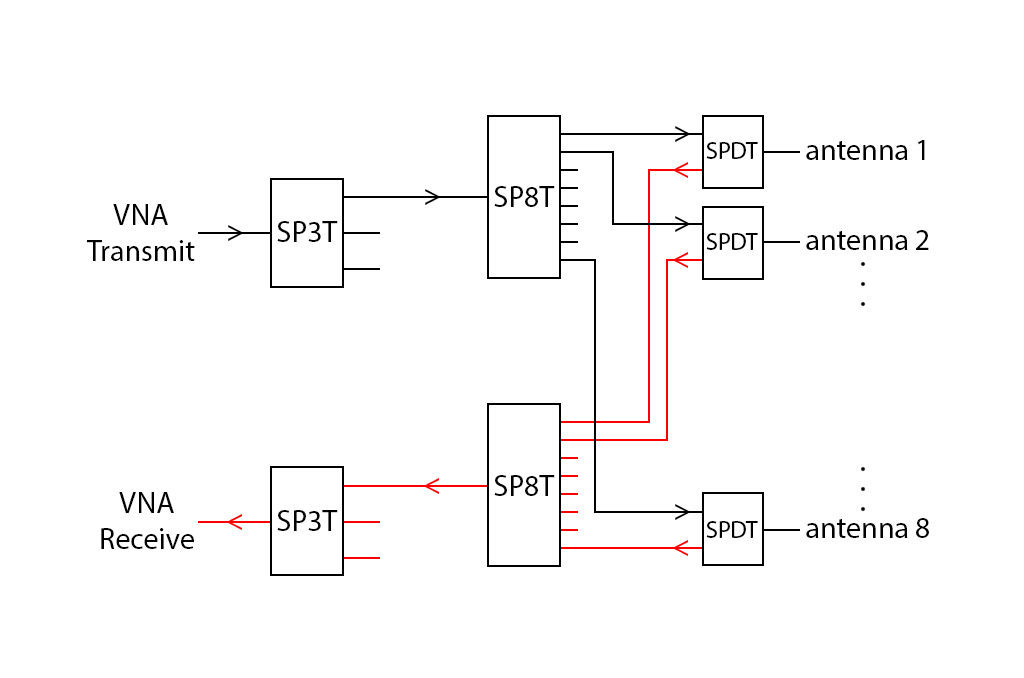
\includegraphics[width=5in]{./images/mp_final_layout.png}
		\caption{Final design of the multiplexer}
		\label{fig:mp_final_layout}
	\end{center}
\end{figure}


With this design decided on, we needed to get it manufactured on PCB. To create the PCB layout necessary to get these boards printed, software package Altium was used. Two boards were designed for the RF portion of the multiplexer; one containing only an SP3T and one containing two SP8Ts and eight SPDTs. The final 2 x 24 multiplexer requires two of the boards with SP3Ts and three of the boards with SP8Ts and SPDTs. The final PCB layout of the two boards is shown in figures \ref{fig:sp3t}, \ref{fig:sp8t_top} and \ref{fig:sp8t_bottom}.

Both boards were designed with 4 layers using a substrate of FR-4. The stack up of the boards consists of a top signal layer, followed by a substrate layer, then an internal signal layer (used only as ground in this design) and then the prepreg layer. Below the prepreg layer is a mirror of what is on top of it; an internal signal layer, then substrate layer and then bottom layer. The stack up from Altium is shown in figure \ref{fig:stackup}. 

Both boards used co-planar waveguides with ground for all of the RF traces and were designed such that they were 50 ohms. This resulted in a trace width of 0.5 mm and a gap of 0.115 mm with a substrate thickness of 0.6 mm. Three 10 pin connectors were added to provide power as well as connect all of the control pins for the SP8T and SPDT switches \cite{rob1}.

 
\begin{figure}[h]
	\begin{center}
		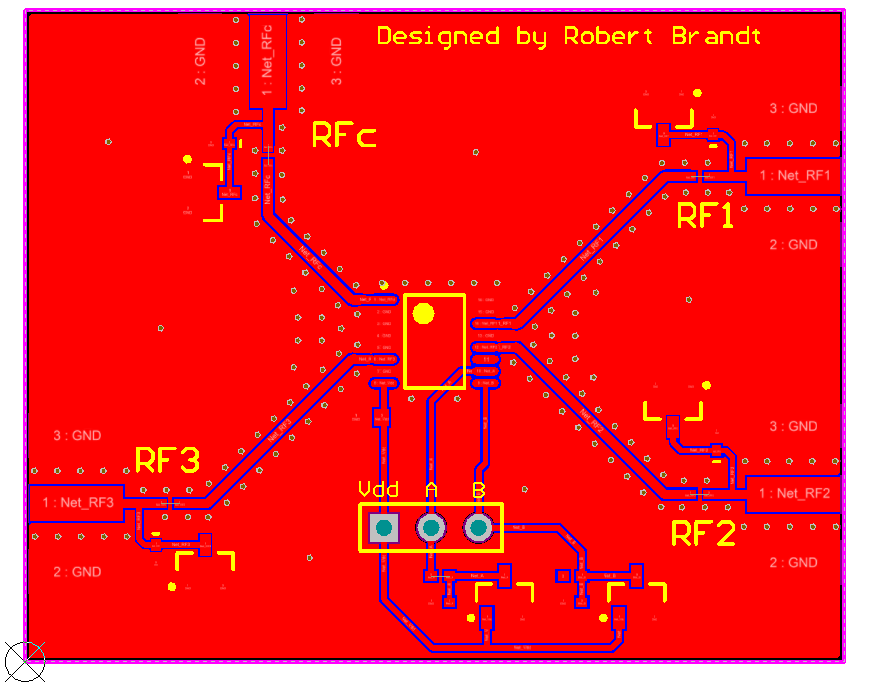
\includegraphics[width=3.5in]{./images/sp3t.png}
		\caption{PCB layout for SP3T board}
		\label{fig:sp3t}
	\end{center}
\end{figure}

\begin{figure}[h]
	\begin{center}
		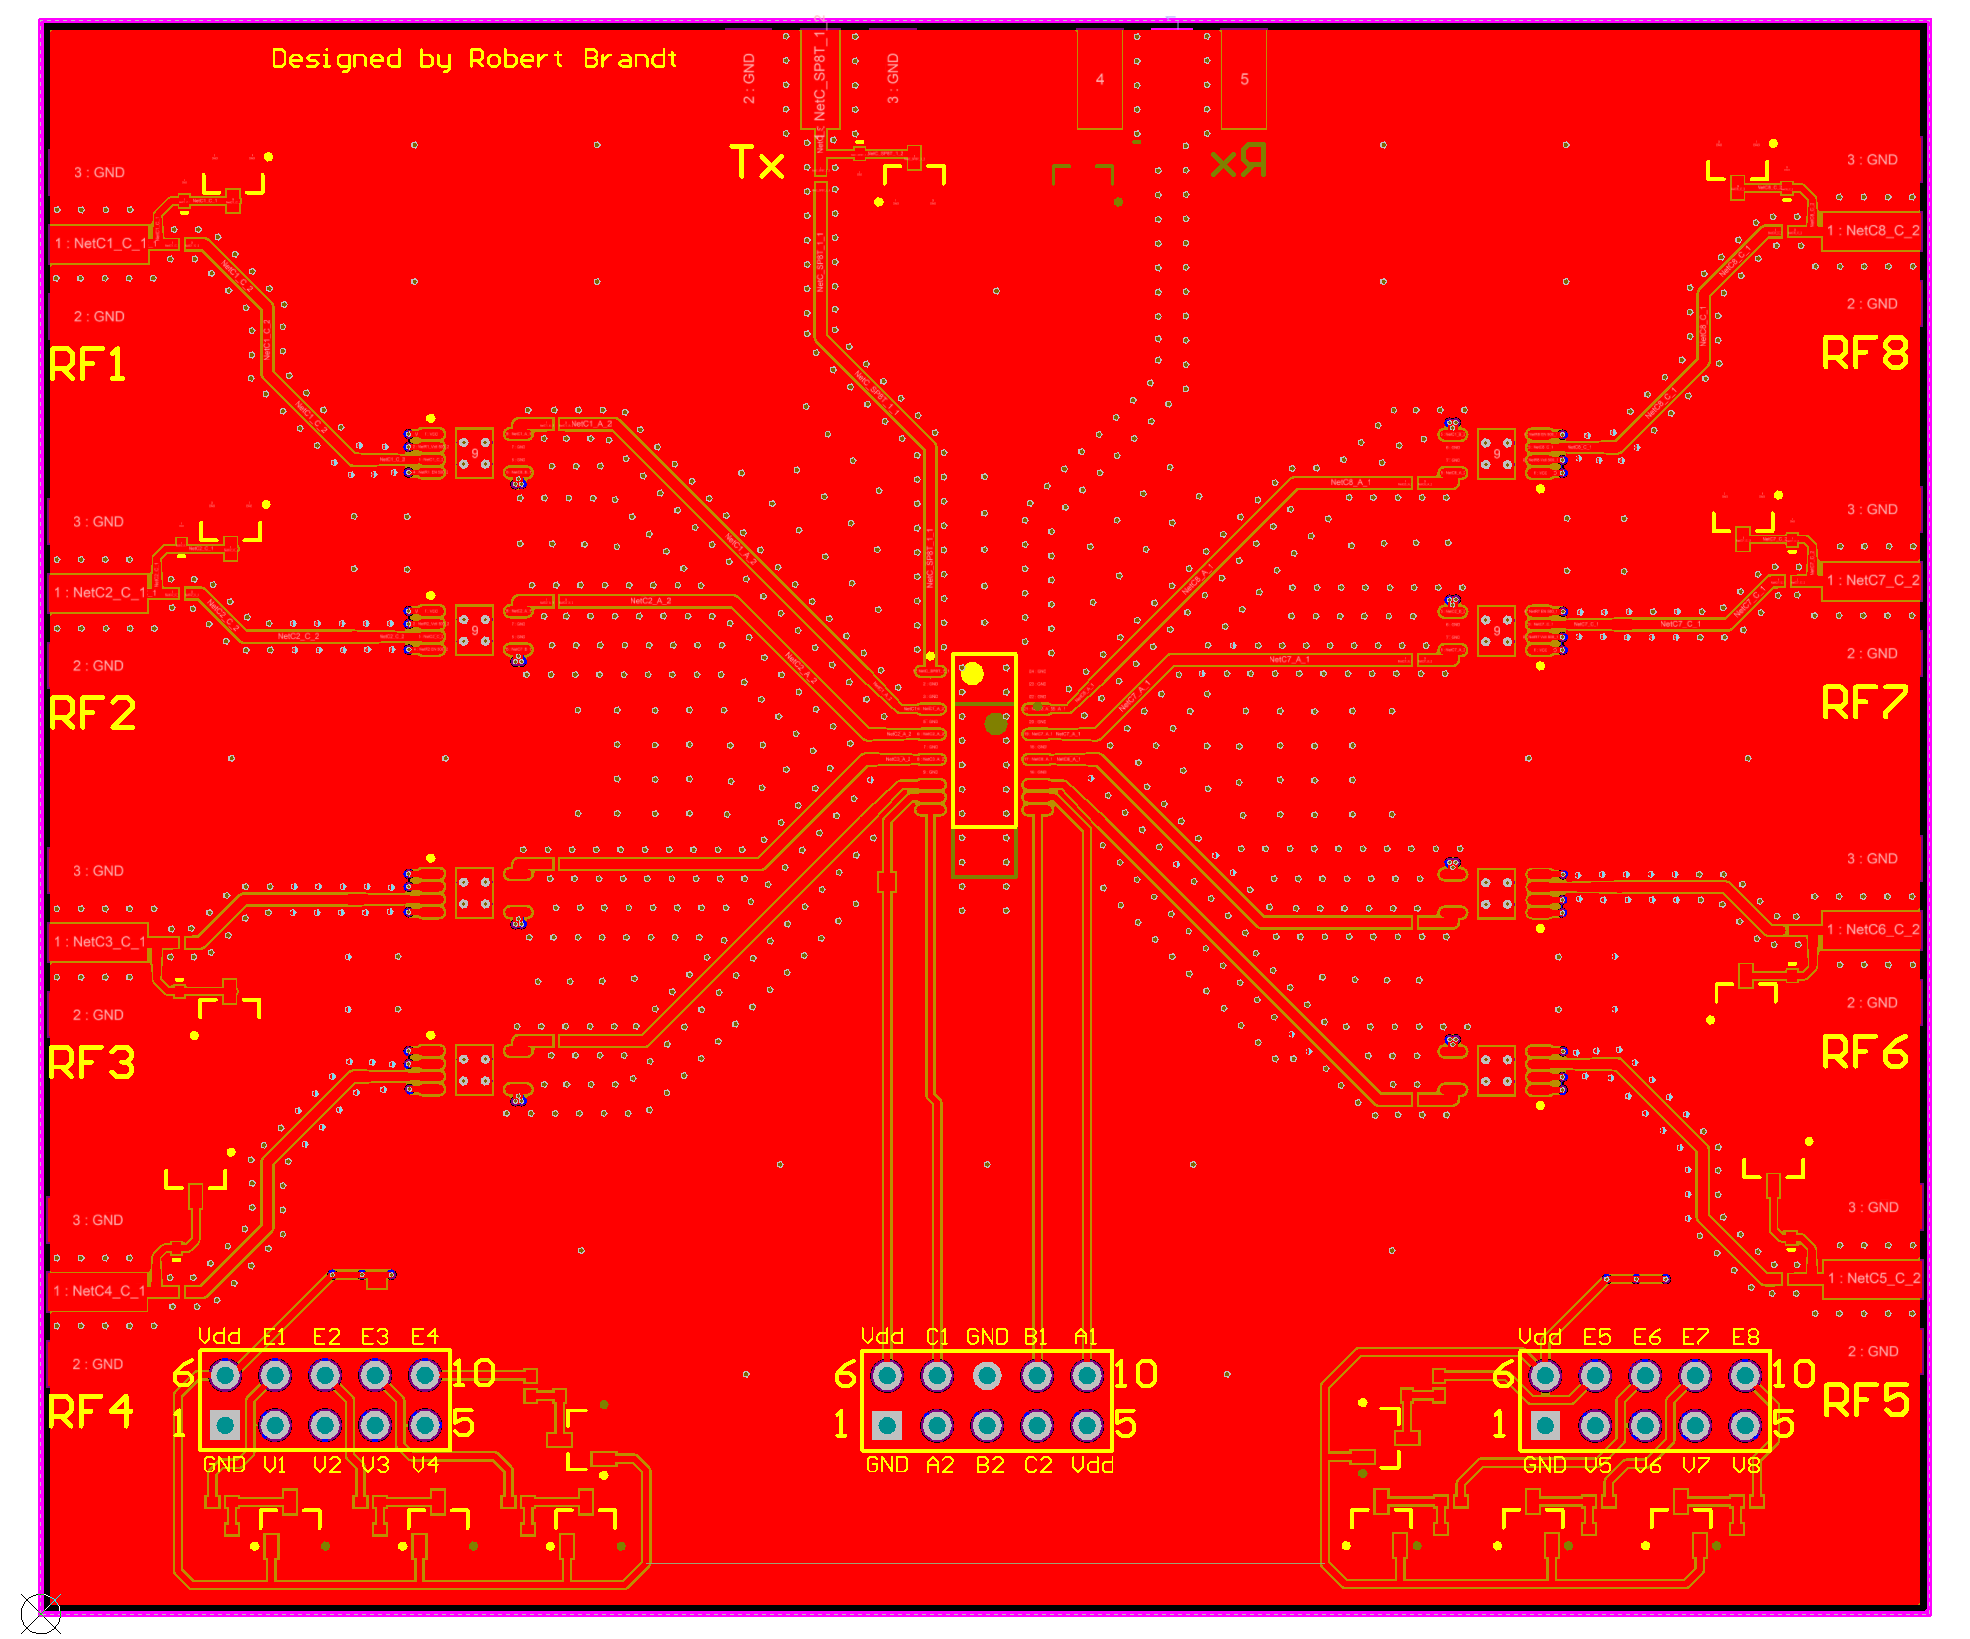
\includegraphics[width=5.5in]{./images/sp8t_top.png}
		\caption{PCB layout for top layer of SP8T and SPDT board}
		\label{fig:sp8t_top}
	\end{center}
\end{figure}

\begin{figure}[h]
	\begin{center}
		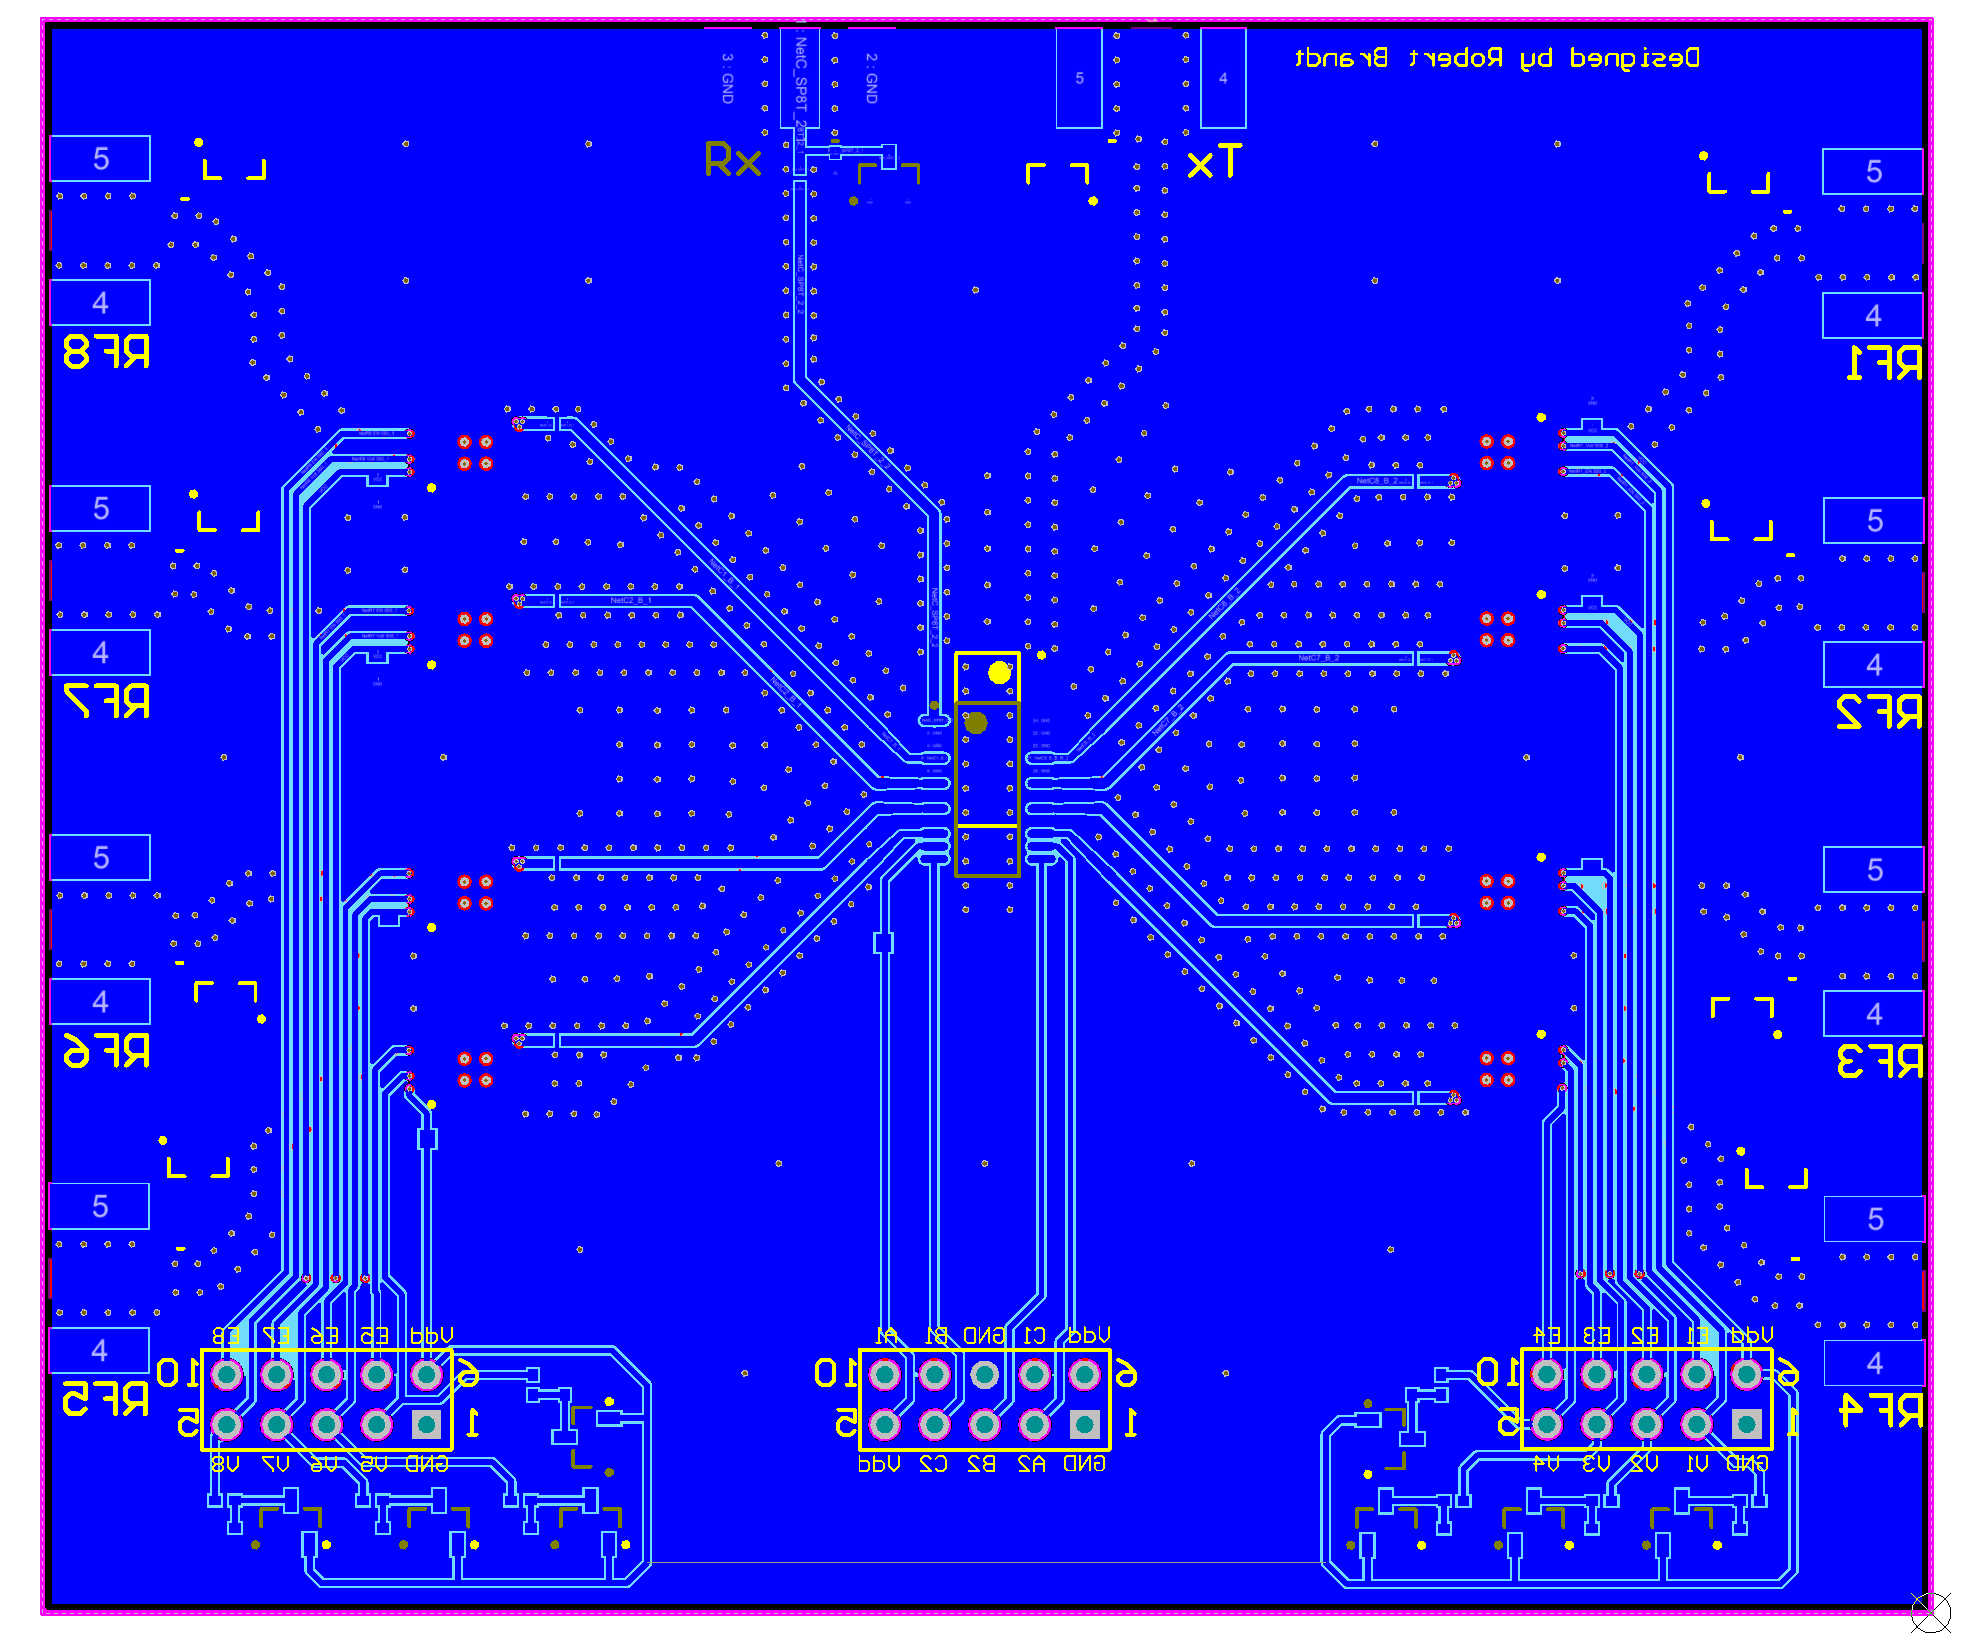
\includegraphics[width=5.5in]{./images/sp8t_bottom.png}
		\caption{PCB layout for bottom layer of SP8T and SPDT board}
		\label{fig:sp8t_bottom}
	\end{center}
\end{figure}

\begin{figure}[h]
	\begin{center}
		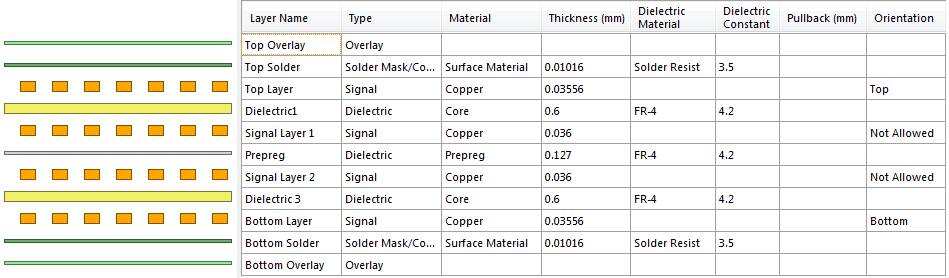
\includegraphics[width=5in]{./images/stackup.png}
		\caption{Stack up for PCBs in Altium}
		\label{fig:stackup}
	\end{center}
\end{figure}


Unfortunately, due to issues with our original intended supplier of our PCBs, we were unable to get these PCBs printed in time for this report. We found another supplier for our PCBs and hope to have them before our presentation. The PCBs needed to be modified somewhat due to different PCB specifications from this new supplier. Minimum routing size was larger at 0.1524 mm compared to 0.1 mm with the original supplier. Also, the substrate thickness options were different, not allowing us to use a thickness of 0.6 mm. Based on the specifications of the new supplier the RF traces needed to be modified to 0.185 mm thick with a gap of 0.1524 mm. This is based on a substrate thickness of 0.1 mm.

